\documentclass[a4paper,12pt]{article}
\usepackage{amsmath, amsthm, amssymb}
\usepackage{datetime}
\usepackage{tikz} % 添加绘图
\usepackage{framed}
\usepackage{tabularx}
\usepackage{enumitem}
\usepackage{fancyref}
\usepackage{csquotes}
\usepackage{wrapfig}

\usepackage[top=1in,bottom=1in,left=1in,right=1in]{geometry} % 用于设置页面布局
\usepackage{xeCJK} % 用于使用本地字体
\usepackage[super, square, sort&compress]{natbib} % 处理参考文献
\usepackage{titlesec, titletoc} % 设置章节标题及页眉页脚
%\usepackage{xCJKnumb} % 中英文数字转换
\usepackage{amssymb}
\usepackage{amsmath} % 在公式中用\text{文本}输入中文
\usepackage{diagbox}
\usepackage{multirow} % 表格中使用多行
\usepackage{booktabs} % 表格中使用\toprule等命令
\usepackage{rotating} % 使用sidewaystable环境旋转表格
\usepackage{tabularx}
\usepackage{graphicx} % 处理图片
\usepackage{footnote} % 增强的脚注功能,可添加表格脚注
\usepackage{threeparttable} % 添加真正的表格脚注,示例见README
\usepackage{hyperref} % 添加pdf书签

\usepackage{tikz}
\usetikzlibrary{shapes,arrows,shadows}

% 字体设置
\setmainfont{Times New Roman}
\setsansfont[Scale=MatchLowercase,Mapping=tex-text]{PT Sans}
\setmonofont[Scale=MatchLowercase]{PT Mono}
\setCJKmainfont[ItalicFont={Kaiti SC}, BoldFont={Heiti SC}]{Songti SC}
\setCJKsansfont{Heiti SC}
\setCJKmonofont{Songti SC}
% \setCJKmainfont[BoldFont={FZXiaoBiaoSong-B05S}]{Songti SC}
% \setCJKfamilyfont{kai}[BoldFont=Heiti SC]{Kaiti SC}
% \setCJKfamilyfont{song}[BoldFont=Heiti SC]{Songti SC}
% \setCJKfamilyfont{hei}[BoldFont=Heiti SC]{Heiti SC}
% \setCJKfamilyfont{fsong}[BoldFont=Heiti SC]{Songti SC}
% \newcommand{\kai}[1]{{\CJKfamily{kai}#1}}
% \newcommand{\hei}[1]{{\CJKfamily{hei}#1}}
% \setromanfont[Mapping=tex-text]{TeXGyrePagella}
% \setsansfont[Scale=MatchLowercase,Mapping=tex-text]{TeXGyrePagella}
% \setmonofont[Scale=MatchLowercase]{Courier New}
%%设置常用中文字号,方便调用
\newcommand{\erhao}{\fontsize{22pt}{\baselineskip}\selectfont}
\newcommand{\xiaoerhao}{\fontsize{18pt}{\baselineskip}\selectfont}
\newcommand{\sanhao}{\fontsize{16pt}{\baselineskip}\selectfont}
\newcommand{\xiaosanhao}{\fontsize{15pt}{\baselineskip}\selectfont}
\newcommand{\sihao}{\fontsize{14pt}{\baselineskip}\selectfont}
\newcommand{\xiaosihao}{\fontsize{12pt}{\baselineskip}\selectfont}
\newcommand{\wuhao}{\fontsize{10.5pt}{\baselineskip}\selectfont}
\newcommand{\xiaowuhao}{\fontsize{9pt}{\baselineskip}\selectfont}
\newcommand{\liuhao}{\fontsize{7.5pt}{\baselineskip}\selectfont}

% 章节标题显示方式及页眉页脚设置
% \item xCJKnumb是自己额外安装的包
% \item titleformat命令定义标题的形式
% \item titlespacing定义标题距左、上、下的距离
\titleformat{\section}{\raggedright\large\bfseries}{\thesection}{1em}{}
\titleformat{\subsection}{\raggedright\normalsize\bfseries}{\thesubsection}{1em}{}
\titlespacing{\section}{0pt}{*0}{*2}
\titlespacing{\subsection}{0pt}{*0}{*1}
% 由于默认的2em缩进不够,所以我手动调整了,但是在windows下似乎2.2就差不多了,或者是article中没有这个问题
\setlength{\parindent}{2.2em}

% 设置表格标题前后间距
\setlength{\abovecaptionskip}{0pt}
\setlength{\belowcaptionskip}{0pt}


\renewcommand{\refname}{\bfseries{参~考~文~献}} %将Reference改为参考文献(用于 article)
% \renewcommand{\bibname}{参~考~文~献} %将bibiography改为参考文献(用于 book)
\renewcommand{\baselinestretch}{1.38} %设置行间距
\renewcommand{\figurename}{\small\ttfamily 图}
\renewcommand{\tablename}{\small\ttfamily 表}


\usepackage{stmaryrd}
\usepackage{mathtools}
\usepackage{csquotes}

\title{有效过程与自然法则}
\date{1985 年 9 月 9 日}
\author{罗伯特·罗森}

\begin{document}

\maketitle{}

\renewcommand\contentsname{目录}
\setcounter{tocdepth}{2}
\tableofcontents

\section{引言}

现代科学史上最引人注目的思想交汇之一,发生在 1931 年哥德尔关于形式不可判定性的原始论文发表与 1943 年麦卡洛克和皮茨关于神经网络的著作发表之间的短短几年间。
在这 12 年中,逻辑学、数学、大脑理论和数字计算的可能性之间建立了基本的相互关系,而真实的数字计算仍然还差让人心动的那么一步来全面实现。人们当时认为,
半个世纪之后的今天依然如此认为,这些思想预示着一场革命,就像三个世纪前牛顿所取得的革命一样。

\begin{figure}[ht]
\centering
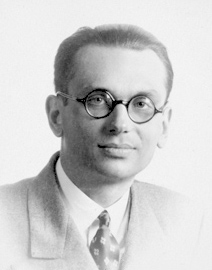
\includegraphics[height=1.5in]{images/kurt_godel.jpg}
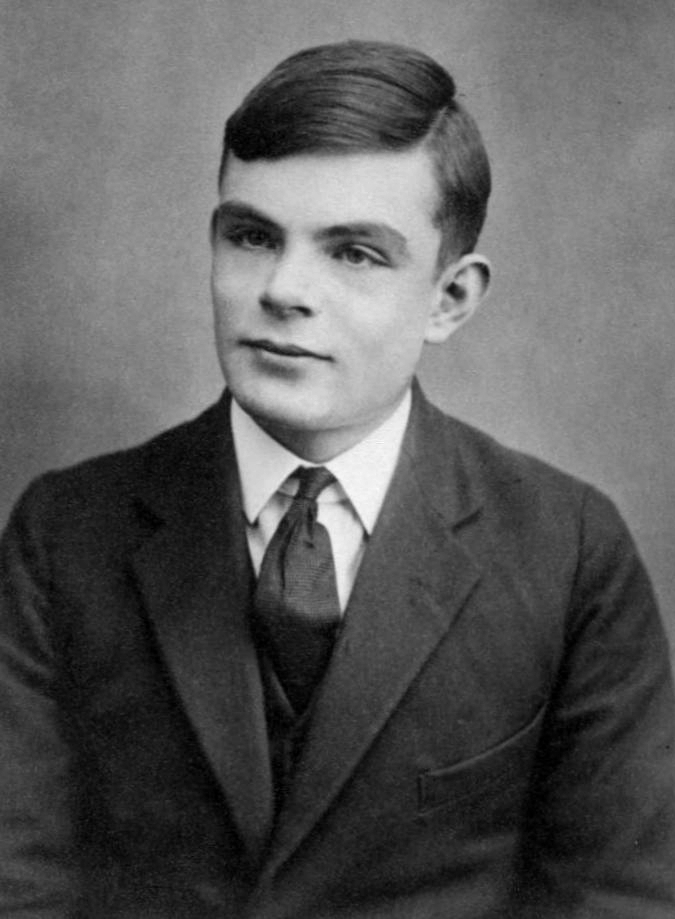
\includegraphics[height=1.5in]{images/alan_turing.jpg}
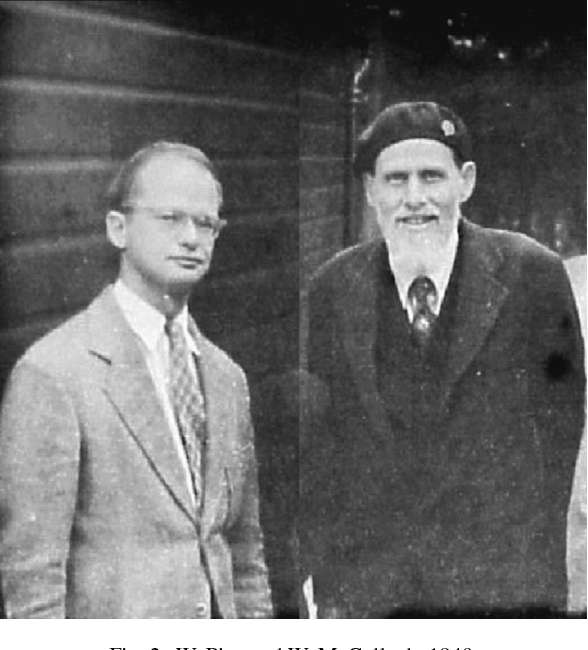
\includegraphics[height=1.5in]{images/pitts_mcculloch_1949.png}
\caption{青年哥德尔;青年图灵;皮茨和麦卡洛克的合照}
\end{figure}

阿兰·图灵的名字在这些惊人发展的历史上是非凡的。正因为图灵,在他 1936 年发表的开创性论文中,通过构建以他的名字命名的“机器”类,他首次把这些相关的思想真正并列在一起。
一方面,图灵机是从人类进行数学计算的心理过程中明确推演出来的;另一方面,它们代表了逻辑或算法过程在数学中的形式化的体现;再一方面,通过使用“机器”这个术语,
它们又代表了,利用物质过程来扩展我们自己的数学能力(很快会通过数字计算机的发明来实现),并且在更深的层次上,为探索生命本身建立一个新的、强大的隐喻。

\begin{figure}[ht]
\centering
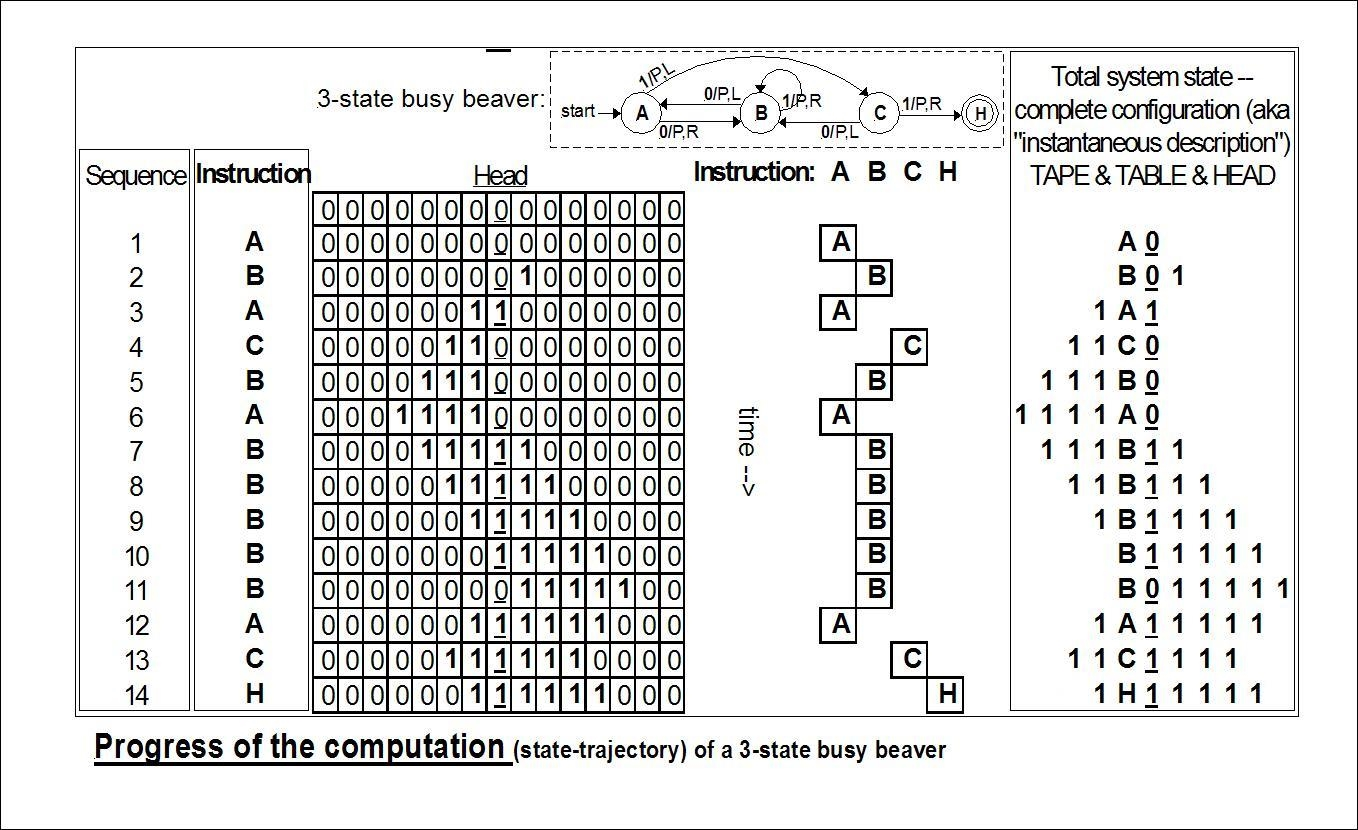
\includegraphics[height=2.0in]{images/turing_machine.jpg}
\caption{图灵机计算忙碌海狸问题的过程}
\end{figure}

在纯粹的数学/逻辑层面上,人们很快认识到,图灵机是体现算法概念的许多等价形式之一。反过来,一个算法被认为是一个解决问题的有效过程的缩影。
首先,一个有效过程意味着一种绝对必要性;它是一个推理链条,对从适当初始数据开始的每一个情况,它都必须要导向相应的那个答案或解答。
此外,算法是一个死记硬背的过程,一旦启动,在从数据到解答的无休止的过程中,不需要进一步的干预、省察和思考。这就是为什么,现在回想起来,
把它体现在一台“机器”上是如此自然,就像图灵做的那样。

\begin{wrapfigure}{r}{0.3\textwidth}
  \begin{center}
    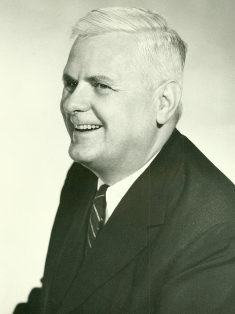
\includegraphics[height=2.0in]{images/alonzo_church.jpg}
  \end{center}
  \caption{阿隆佐·邱奇}
\end{wrapfigure}

由于“有效过程”的概念是一个非形式的、直观的概念,而“算法”的概念是一个精确的形式化的数学概念,早期有人提出后者可以取代前者。
这正是邱奇论文(参见 Kleene1952)的实质内容, 该论文断言,任何人们想称之为“有效”的过程,已经可以通过一些适当编程的图灵机器来完成。


现在,严格地说,到目前为止所描述的所有讨论都是完全形式化的;它们发生在命题和产生规则的逻辑和数学宇宙中。从某种意义上说,它们都是“软件”。
然而,有趣之处主要集中在这样一个事实上:像“机器”或“有效”这样的术语具有非数学的内涵,这些内涵都属于自然物质现象的外部世界。
事实上,正如我们已经注意到的,图灵自己设计的数学机器是从现实世界的现象中抽象出来的,一个人在进行计算。这种暗示如此不可抗拒地传达出,
如果人类精神活动的这一方面可以“机械化”,为什么其他方面不可以呢?为什么不可以是全部呢?同样地,如果心理过程,包括在物质大脑中发生的事情(也即在硬件中)可以完全形式地表示,
为什么不能有其他类型的物质系统(也即其他硬件)可以做与大脑相同的事情?虽然还在胚胎阶段,在这里,我们看到了,“人工智能”的最广推论,以及许多其他的意涵。

但是,一旦我们承认“机器”或“有效”这样的词具有物质意义,我们就离开了数学的世界,进入了(最广义的)物理世界。正如我们已经提到的,图灵机是“纯软件”,
而物理学则相反,是“纯硬件”。因此,无论是好是坏,我们引入了硬件和软件之间的根本区别,它本身并不是我们开始时所使用的形式理论的一部分;同样,它也不是物理学的一部分。
正如我们将要看到的,这种区别是至关重要的,但是它是一种隐蔽的危险,藏在包罗万象的总称“机器”中。从马丁·戴维斯 1958 年出版的《可计算性和不可解性》一书中,
我们可以看到这种区别是如何悄无声息地出现的:

\begin{displayquote}
    我们怎么能排除某一天(也许是某个外星访客)给我们一个(也许是极其复杂的)设备或“神谕”来“计算”一个不可计算函数的可能性呢?
\end{displayquote}

这显然是在一个完全形式化的数学发展背景下提出的最具修辞性的反问句。但是我们在这里清楚地看到术语“机器”的任意性,它建立在真实硬件和逻辑软件之间的默认区别之上。

\begin{figure}[ht]
\centering
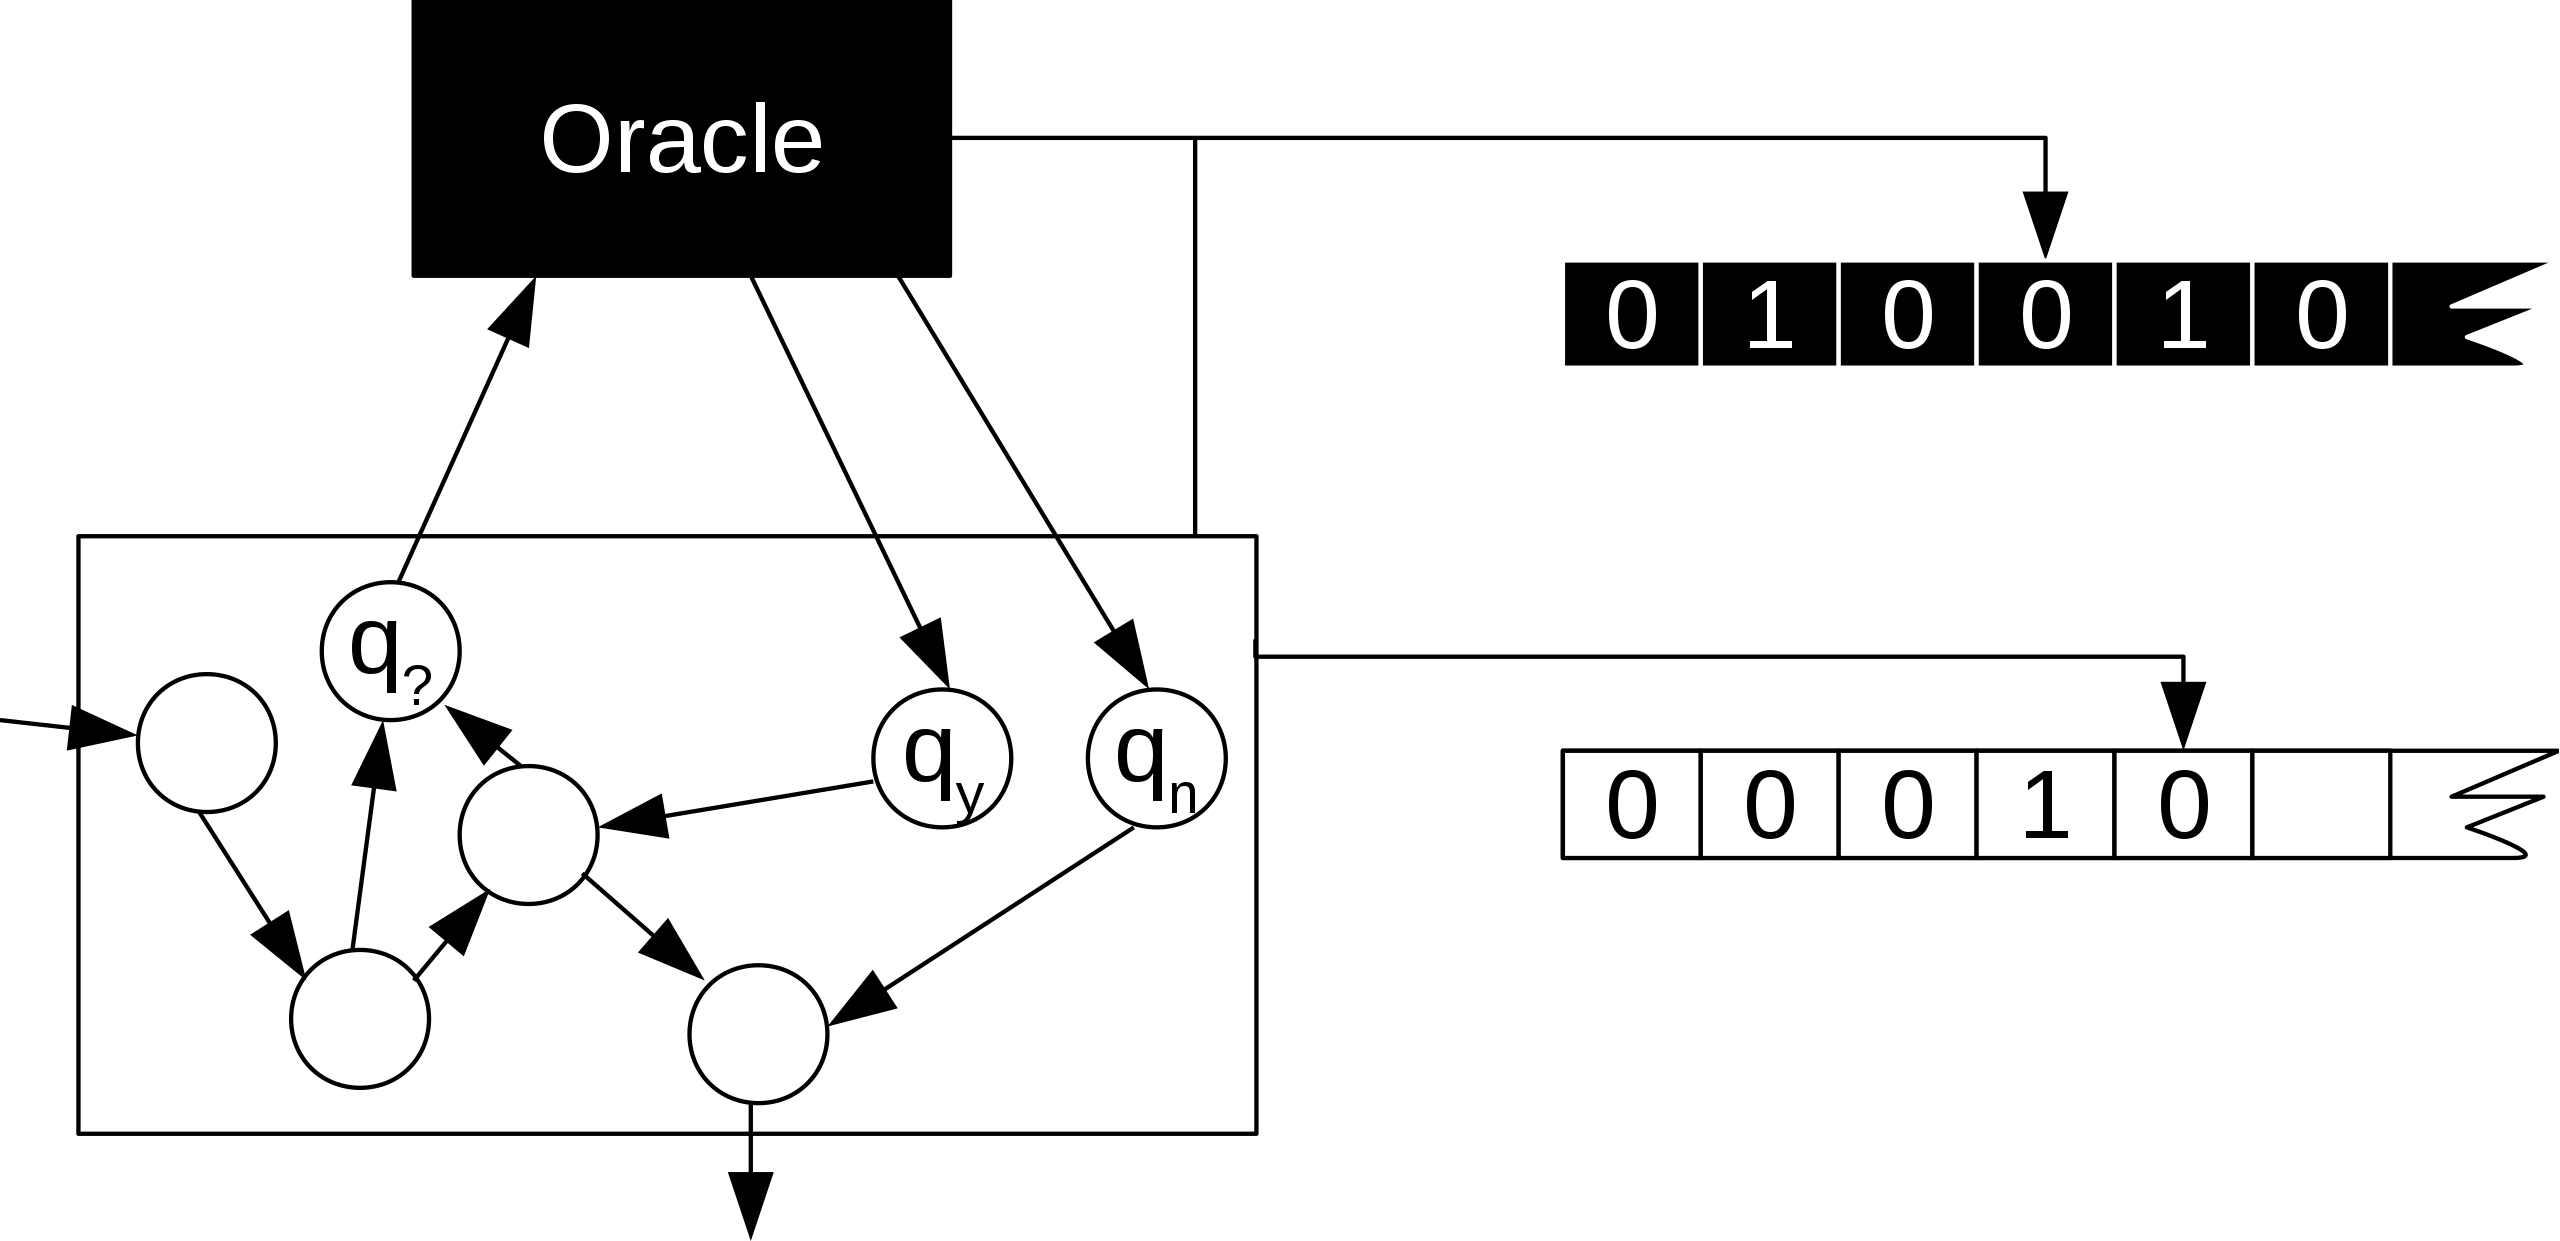
\includegraphics[height=2.0in]{images/turing_machine_oracle.png}
\caption{带神谕的图灵机}
\end{figure}

长期以来,作者一直为这一问题的深层认识论的结论所困扰。特别是,一旦我们承认“硬件”或物质系统进入我们的讨论(正如我们已经指出的那样,这从一开始就是明确无误的意图),
那么“有效过程”的概念会发生什么变化呢?很久以前(Rosen 1962),我考虑的问题是邱奇的论点在这个新的背景下意味着什么。
特别地:邱奇的论点是否是对物质本性的一个基本限制呢(类似于热力学定律排除了永动机),或者相反? 如果邱奇的论点可以被自然过程破坏,那么递归性又会怎么样呢?

在这里回顾一下先前论点的要点可能是有用的。假设我们有一个物理系统 $S$(也许是戴维斯的外星“计算机”)。它的行为受到物理定律的支配,我们通过实验来了解这些定律。
一个典型的实验要么对系统做一些事情(例如,从外部扰动它),要么让系统对其环境做一些事情,然后观察或测量结果。显然,实验者的干预和测量的结果都是物质事件。
事件是由数字来描述或刻画其特性的,其数值是由应用的合适的量表来决定的(参见 Rosen1978)。为了简单起见,假设我们的实验干预 $\alpha$ 拥有的属性是这样一个数值 $r(\alpha)$,
而我们系统的结果行为由另一个这样的数字刻画。通过这种方式,我们的实验者可以生成一个数值表,它定义了一个从数字到数字的函数 $f$。
$$
r(\alpha) \mapsto \beta
$$

读者将会认识到,这个过程以典型输入输出的方式刻画了我们系统 $S$。函数 $f$ 的形式,清楚地告诉我们支配 $S$ 行为的规律。毕竟,这就是科学实验的全部功能。

这个实验过程在某种意义上是有效的。事实上,正如我们将在下面详细论述的那样,物质世界(例如,在系统 $S$ 中)的事件序列是由因果关系所支配的,这些因果关系将它们联系在一起,就像蕴涵关系将命题无可避免地联系在一起一样。
因此,如果我们的实验过程是可重复的(这意味着 $S$ 中相同的因果序列可以随意重建) ,那么邱奇的论点必须意味着任何输入输出函数 $1$,正如我们已经描述过的任何物质系统 $S$,也必须是递归的或可计算的。
否则,系统 $S$ 将正是戴维斯向我们保证排除在可能性之外的那种“计算机”。

从这个角度来看,邱奇的论文试图从软件(算法)的前提中得出关于硬件(物理学)的推论或结论。
冯 · 诺依曼关于“自我复制”的论点(Burks 1966; Arbib,本卷; 参见下文第5节)体现了另一种众所周知的同样尝试。
在这里,我们的目的是从一个关于计算的形式理论中学习关于物质系统(特别是有机体)的行为的一些东西。
不出所料,这类尝试风险极大,但如果能成功实现,回报将是巨大的。

\begin{figure}[ht]
\centering
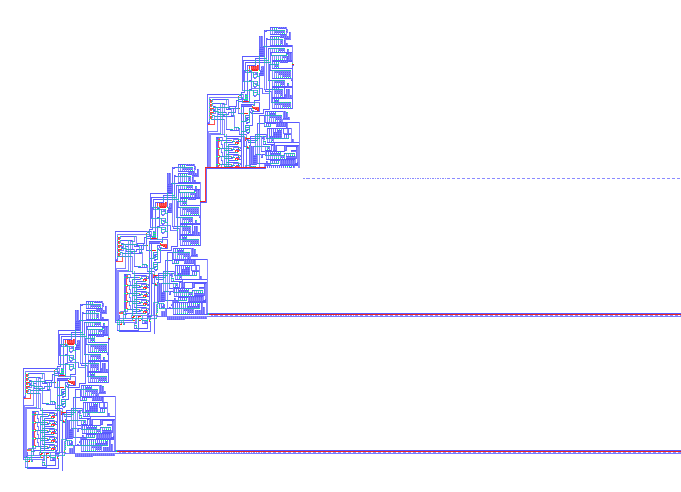
\includegraphics[height=2.0in]{images/self_reprod.png}
\caption{运行中的第一个为人所知的自复制机}
\end{figure}


至少,我们可能已经看到,在形式理论中引入“硬件”的概念将产生一些特殊的结论。而当我们试图把“软件”的概念引入物理学时,互补的结论就出现在另一方面。
然而,这些特殊的结论将告诉我们一些关于这两者的有趣事情。在本文的其余部分,我们将探索这种可能性。

\section{形式系统中的邱奇论题}

邱奇论题的实质是,把任何形式系统中的逻辑推理与字符串处理等同起来。反过来,字符串处理或字处理是一种纯粹的语法活动。
当然,字符串处理正是图灵机所做的。尽管如此,从表面上看,这似乎是一个非常强的、或许有些过于强的条件,
它要求形式系统中的每一个推理,都应该只用语法项来表达;也就是说,从前提到结论的每一个步骤,都应该完全通过,对这些编码了的命题的符号进行操作来实现。

Nevertheless, a rather strong case can be built to support this rather
unlikely-looking Thesis. It distills a trend towards formalization which
began with Euclid, became a matter of urgency in the confusion following the
discovery of non-Euclidean geometries (i.e., geometries which, as formal
systems, were consistent as God-given Euclid), and of absolute desperation
when the paradoxes in naive set theory were revealed. The formalistic response
to this situation, pioneered by David Hilbert, was precisely to empty
mathematics of any semantic content whatsoever, arguing in effect that it
was a needless semantics which was at the root of the difficulties.
This in effect turned all of mathematics into a kind of game in which meaningless
symbols were manipulated according to (a finite family of) arbitrary syntactical rules.
Indeed, the whole point of Hilbertian Formalism is to create systems in which there is
nothing but syntax.

Perhaps the clearest statement of this kind of Formalist program was given by Kleene 1952:

\begin{displayquote}
This step (axiomatization) will not be finished until all the properties of the
undefined or technical terms of the theory which matter for the deduction
of theorems have been expressed by axioms. Then it should be possible to
perform the deductions treating the technical terms as words in themselves
without meaning.  For to say that they have meanings necessary to the deduction
of the theorems, other than what they derive from the axioms which
govern them, amounts to saying that not all of their properties which matter
for the deductions have been expressed by axioms. When the meanings
of the technical terms are thus left out of account, we have arrived at the
standpoint of formal axiomatics \ldots Since we have abstracted entirely from
the content matter, leaving only the form, we say that the original theory has
been formalized. In this structure, the theory is no longer a system of meaningful
propositions, but one of sentences as sequences of words, which are
in turn sequences of letters.  We say by reference to the form alone which
combinations of words Itre sentences, which sentences are axioms, and which
sentences follow as immediate consequences of others.
\end{displayquote}

Clearly, the idea here is that it is always possible to replace semantics ("meanings")
with syntactics, so that logically no information is lost; any inference involving semantics
possesses a purely syntactical image in the formalization.

In such a formal system, we start with the idea that the axioms are true.
This notion of truth is hereditary; if the axioms are true, then so also are the
symbol sequences obtained by applying the inferential rules of the system to them;
thus truth passes from axioms to theorems. So far, we never need to import a notion of "truth"
into the system from outside, as it were; we simply construct true propositions (theorems)
as we go along.

The troubles embodied in Gliders celebrated theorems (GOdel 1931)
arise from trying to compare this constructive notion of internal truth with
preassigned external truth-value in formal arithmetic; as Godel showed, they
do not match. Furthermore, one way of looking at Turing's theorem on decidability (Turing 1936-7)
is that there is no internal inferential mechanism for deciding whether a proposition
in the given formalization is a theorem(i.e., true) or not. Thus, we know that the Formalist program,
in which only purely syntactic inferences are allowed, is too impoverished to even play the game of number theory.
That is, we must either allow into our system some "informal" inferential procedures, which according to Godes Theorem
cannot be reduced to syntactics even in principle, or else restrict ourselves forever to mere fragments of number theory.
Such "informal" inferential procedures are what are disallowed by Church's Thesis; they are ineffective.

Let us put the above discussion into more familiar terms. In ordinary
("Platonic") mathematics, which of course has both a syntactic and a semantic aspect,
we know that if we are given a set, a variety of other sets
can always be built from S via canonical constructions. For example, we
have the power set 28; we have the free algebraic structures (semigroup,
group, etc.)  generated by S, we have the set H(S, S) of all maps from
S to S; we have the Cartesian product S x S, etc. These associated sets
give us inferential capabilities which have the power of logical relations,
without necessarily being expressible in terms of the formal inferential laws
which govern the mathematical system from which S came. For instance,
if Q : S 	S is an automorphism of S (i.e., an element of H(S, S)), and
s E S, we may say that Q(s) = s' establishes an implication relation between and s'.
But this "implication" need not coincide with any we can draw
from the production rules governing the system; i.e., need not follow from
system syntactics alone. If it does, we may say that our Q is computable in
the system; otherwise, not computable. In the latter case, we would have to
say that the mapping Q is not effective, according to Church's Thesis. But
clearly, if Q has any meaning or existence at all, once it is given to us, it is
effective.

In the "all-software" world of formal systems, we can of course restrict ourselves in any way we like.
Thus, we can agree not to allow ourselves any automorphisms Q which cannot be expressed in purely syntactical
terms. In such a world, and only in such a world, could Church's Thesis hold unrestrictedly.
Whether such a formal world would be at all interesting is, of course, another question.
And as we shall see, the situation gets even worse when we allow "hardware" into our world.

Before turning to material systems, we should say a word about the encoding of propositions
in a formal system onto Turing machine tapes, and decoding tapes back into propositions in the system.
It is fairly clear that we may use the word "effective" in its usual intuitive sense in connection
with encoding and decoding; the familiar Godel numbering, for example, is
clearly an effective mapping from syntax to arithmetic and back. Indeed,
in showing that a process in some formal system is effective, or recursive,
we can clearly combine the encoding, the computation, and the decoding
into a single Turing machine which does all three. However, we merely note
here for future reference that the encoding and decoding are logically distinct from each other
and from the actual computation; if these are in some sense "ineffective", then Church's Thesis
may appear to fail, even though the computation itself is completely recursive.

\section{蕴含与因果性}

As we have seen, in the realm of formal systems, Church's Thesis identifies the intuitive notion of "effective process" with the purely syntactic idea of string processing.

That is, any implication which can be "effectively" performed within the system can already be carried out by means of a finite set of production rules,
operating on finite strings of symbols taken from a f i nite alphabet. We have also pointed out that when we deal with the material world
(as opposed to the formal ones of mathematics and logic) ideas of implication are replaced by ideas of causality. Nevertheless, we can still
retain the idea of an "effective" process. In this context, Church's Thesis means that any causal sequence can be represented by a corresponding
recursive process; i.e., any causal sequence can be described by purely syntactic means. If this is true, it of course places severe
limitations on what physics can be like. The question is no less than whether the Laws of Nature can themselves be formulated in purely
syntactical terms, or whether they can possess an inherent semantic component which cannot be finitistically formalized.
It should be noted that the urge to formalization (i.e., to pure syntactics) in mathematics is exactly parallel to similar trends in theoretical science.
Indeed, the whole thrust of atomic theory (or nowadays, the theory of "elementary particles") is to reduce all material processes to the motion of
ultimate constituent units, devoid of any internal structure ("meaning"), possessing only an instantaneous position ("configuration")
and the temporal derivatives of position. The forces which push these ultimate units around are the precise analogs of the production rules in a formal system.
Hence the paths or trajectories traced out by a material system under the influence of given forces are the analogs of formal theorems,
with initial conditions as axioms. The idea that causal relations between events in material systems can be related to implication relations between
propositions describing those events is the sine qua non of theoretical science. Indeed, the belief in what used to be called Natural Law requires (a)
that the sequences of events we perceive in the external world are not arbitrary or whimsical, but are governed by definite rules (this is Causality),
and (b) that these rules can be articulated in such a way that they can be grasped by the human mind. Taken together, this formulation of Natural Law
asserts precisely that causal relations in material systems can be brought into congruence with implications in a
formal (ultimately, mathematical) system of propositions about those events.

This situation can be most succinctly expressed in terms of a diagram (see Figure 1).

We say that a modeling relation exists between the natural system on the left of the diagram, and the formal system on the right, when the following

commutativity holds:
0 = 02 + 0 + 	(1)
That is, we get the same answer whether we simply sit as observers, and watch the unfolding sequence of events in the natural system, or whether we (a) encode some properties of the natural system into the formalism, (b) use the implicative structure of the formal systhm to derive theorems, and then (c) decode these theorems into propositions (predictions) about the natural system itself.  When the diagram commutes, we have established a congruence between (some of) the causal features of the natural system and the implicative structure of the formal system. We can then say that the formal system is a model of the natural one, or alternatively, that the natural system is a realization of the formal one.
   These little diagrams themselves possess a number of rich and important epistemological properties, which we cannot enter into here; for a fuller discussion, see e.g. Rosen 1985.
Once we have thus constructed a formal system which is a model for
some natural process, we have left the realm of science and entered that
of mathematics. We can then treat a model as we would any other formal
system. In particular, we can look at its purely syntactic aspects, which we can immediately identify with the "effective" processes of Church's Thesis,
and ask whether these exhaust the implicative resources of the system itself.

In this way, we can construct a purely syntactic "machine" model of our original natural system, as indicated in Figure 2.

This can be seen by looking only at the outer two systems, and forgetting about our original model, which now plays the role of a "transducer"
between them.

However, when we do this, the following points must be explicitly noticed: (a) the encoding and decoding arrows between them (the
dotted arrows in Figure 2) cannot be described as effective in any formal
sense, and (b) these encoding and decoding arrows involve exclusively the
input and output strings of the machines inhabiting the right-most box. Both
of these observations are important. We shall briefly discuss them each in
turn.

In applying Church's Thesis to formal systems, we noted above that the
corresponding encoding and decoding arrows themselves represented formal processes, which could in fact be amalgamated into
the Thesis itself. However, when we wish to compare a natural system, governed by causality, with a formal system, governed by
implication, this is no longer the case. The encoding instruments, or transducers, are now themselves material systems;
i.e., governed by causality and not by implications. As noted above, they are (in the broadest sense) meters. Since these meters are governed by
causality, anything they do is effective in a material sense. But it is clear that a formalization of the encoding process would require more models;
these would in turn require their own encoding and decoding processes, which would require more models, etc., an infinite regress.
It is precisely this fact which makes "the measurement problem" so hard in physics. The question as to whether this potential infinite regress
can be terminated at some finite point is a deep epistemological question about the nature of the world, with close ties to such things as
reductionism. We cannot of course enter into such matters here; we will merely assume that a set of meters or other transducers
from the natural world to input tapes is given, and that Church's Thesis can be investigated relative to these encodings
(which are then, by hypothesis, effective in the material sense).

Our second observation is also epistemologically important. It says that
all relevant features of a material system, and of the model into which it
was originally encoded (cf. Figure 1), are to be expressed as input strings to
be processed by a machine whose structure itself encodes nothing. That is to
say, the rules governing the operation of these machines, and hence the entire
inferential structure of the string-processing system themselves, have no
relation at all to the material system being encoded. The'only requirement
is that the requisite commutativity hold, as expressed in Section 1 above,
between the encoding on input strings and the decoding of the resultant
output strings. As we shall see, this is the essence of simulation.

We have already noted that Church's Thesis amounts to asserting that
all causal relationships can be expressed in purely syntactic terms. We can
formulate the Thesis still more sharply now: relative to any given encoding
of a natural system into input strings, the string-processing machinery itself
must not encode any aspect of the material system.  That is to say, the
"hardware" of the machines must be totally independent of the "hardware"
generating the strings to be processed. If this cannot be done, then Church's
Thesis cannot be true.

Given the above, Church's Thesis asserts that the Turing machines constitute
a class of universal simulators for all material processes. There are
then two questions to be asked: (a) is it true? and (b) if so, what does it
mean?

\section{邱奇论题在物理上是正确的吗?}

The upshot of the argument of the preceding sections is the following. Na-
ture provides us with a plethora of material processes which we would want
to call "effective". These processes are (we suppose) governed by causality,
and not by implication or production rules, as in a formal system. In these
terms, Church's Thesis can be expressed as follows. Given any such process,
we can encode appropriate propositions about the natural system generating
it onto a set of input tapes to a Turing machine; and the corresponding output
tapes can be decoded so as to perfectly simulate the process in question.
Equivalently, Church's Thesis asserts that all "information" about material
processes, and hence all of Natural Law, can be expressed in purely syntactic
terms.

We know from Gliders Theorem that sufficiently rich formal systems
always contain inferences which cannot be obtained syntactically.  More
specifically, given any encoding of propositions of the system onto input
tapes to Turing machines, there will be propositions of the system which are
"true" but will never appear on any output tape. The processes by which the
"truth" of such inferences are established are thus ineffective; they cannot
in principle be simulated by any Turing machine in the given encoding. We
can always change the encoding, of course, but this will not change Gliders
conclusion.

Thus, in formal systems, we already find that a purely syntactical encoding
will in some sense lose information. The information lost must then
pertain to an irreducible, unformalizable semantic component in the original
inferential structure. By changing the encodings, we can shift to some
extent where this semantic information resides, but we cannot eliminate it.

By itself, this result of Godel does not bear on the physical truth of
Church's Thesis, since it is a purely formal result. But it is in fact suggestive
of how the physical font of Church's Thesis might be verified or falsified.

As we have seen above, the manner in which we compare material processes with formal ones is through the establishment of
modeling relations, as diagrammed in Figure 1 above. Formal models of material systems are
then perfectly good formal systems, whose inferential structures by definition reflect causal processes in the natural system being modeled.
Thus, if a model, arising in this fashion, should fall within the purview of Gliders
argument, this would at least be strong evidence that Church's Thesis is
false as a physical proposition. Stated another way, there would exist physical processes which could effectively compute
nonrecursive functions. It would also mean that Natural Law cannot be expressed entirely in syntactical terms.

The obvious thing to look for, then, is a model of a material system
which is rich enough as a formalism to "do arithmetic". The formalisms
which physics provides, as models of purely physical systems, are unfortunately
extremely impoverished, considered simply as formal systems. But,
as we have argued elsewhere, these formalisms are in fact highly nongeneric
and do not suffice to image material systems like organisms (cf. Rosen, in
press). One way of expressing this nongenericity is precisely in terms of the
way they image causal structures. When this nongenericity is lifted, a new
class of (potential) models is obtained in which the image of causal structure
is infinitely richer and more complicated. Since it is precisely the formal
imaging of causal structures which is at the heart of Church's Thesis, we may perhaps find in these formalisms many processes
which are causally effective, but mathematically ineffective. This would mean that the behavior of such systems must contain
an irreducible semantic component, one intimately related to the complexity of the system.

A different approach was taken long ago by John Myhill (cf. Myhill 1966).
He was able to show that, modulo some idealizations regarding measurement and performance tolerances, there are already
classical analog devices(analog computers) which could "compute" nonrecursive functions. Such systems would thus already
manifest behaviors which could not be predicted by any purely syntactic encoding, and hence would also have an irreducible
semantic aspect.

Finally, we have already mentioned that Newtonian particle mechanics, and more recently, the unified physical theories based on elementary particles,
are in themselves an attempt to express the Laws of Nature in purely syntactic terms. Insofar as any material system is comprised of such "meaningless"
(i.e., structureless) elementary subunits, these theories at heart assert that to understand any behavior of any
such system it suffices to describe it in terms of these subunits and their interactions. As noted earlier, this is the essence of reductionism.

In these terms, the familiar Laplacian Spirit is a purely syntactical concept: the embodiment of Church's Thesis if he could exist.  As a matter
of fact, he could not exist (or at any rate, not as a material system built of particles himself), for reasons we have already indicated.
But even if he could exist, he would be a very poor biologist, for example; organisms, and open systems in general, are constantly turning over their
constituent particles. Thus, to even find an organism, let alone follow it in time, he would need to supplement his purely syntactical
information with other (semantic) information not formalizable within his system.

Thus, for a variety of reasons, there is cause to believe that Church's Thesis fails as a physical proposition. Nevertheless,
as we have seen, to state and analyze the Thesis in material terms touches on some of the deepest and most basic aspects of theoretical science.

\section{模拟的角色}

We have already alluded above to the use of the Turing machines both
as metaphors for the material world and as effective descriptions of that
world.  In both cases, though in different ways, we seek to draw conclusions
about material processes from a purely syntactic formalism. In this final section,
I will very briefly consider one well-known example of this:
the "self-reproducing automata" of von Neumann (Burks 1966; Arbib, this volume).

The basis of von Neumann's argument was the inference of the existence of a "universal constructor" from Turing's
argument for a universal simulator (computer).  On the purely formal side, von Neumann constructed
a universe ("cellular space") of intercommunicating Turing machines arranged along some regular geometric array,
like the cells in a multicellular organism, or ,the neurons in a brain, or atoms in a crystal. Each machine
communicates with its nearest neighbors in the array. In the obvious fashion, the array as a whole changes "state" in time.
The question was whether some sub-array ("tessellation automaton") could induce certain interesting behaviors in its complement,
which could be interpreted as construction, replication, growth, development, evolution, and so on.

At the same time, von Neumann clearly believed that a "universal constructor" could exist as hardware. He envisaged equipping a Turing machine
with sensors, so that it could "read" a blueprint, and with effectors,
so that it could extract physical components from its environment, and
assemble them as instructed by the blueprint being read. (An "effector",
in this context, is a transducer from numbers to things, i.e., an "inverse
meter".) The idea was -that both computation and construction were algorithmic processes,
and therefore whatever was true of the one must be true
of the other.

Von Neumann also felt that the cellular spaces were not merely formal constructs, but actually comprised models of real-world
constructors and their activities. In this, he was tacitly assuming Church's Thesis in its strongest form.

We have argued elsewhere (cf. Rosen 1985), on grounds of causality, that
any inference regarding a material universal constructor from the existence
of a formal universal computer is unjustified.  In that argument, we essentially
showed that there was no intrinsic way of distinguishing between
those input strings which encode "real-world information" and those which
do not. Thus there was no way to distinguish between a computation which
could be claimed to simulate a "real-world" process, and one which has no
such realization.

Conversely, we can also see that the falsity of Church's Thesis means that there are aspects of material processes which cannot be formalized with any given encoding.
Thus there are (a) formal constructions without material counterpart, and conversely, (b) m material constructions without formal counterpart.
Therefore, on both counts, von Neumann's argument is without material content, and merely involves the familiar equivocation on
the terms "automaton" (or "machine") and "construction".

These considerations show how dangerous it can be to extrapolate unrestrictedly from formal systems to material ones.
The danger arises precisely from the fact that computation involves only simulation, which allows the establishment of
no congruence between causal processes in material systems and inferential processes in the simulator. We therefore lack precisely
those essential features of encoding and decoding which are required for such extrapolations. Thus, although formal simulators can be of
great practical and heuristic value, their theoretical significance is very sharply circumscribed, and they must be used with the greatest caution.

There are, of course, many other ramifications of Church's Thesis which we cannot touch on in this brief space. Its main role, as we have seen,
is to separate out what is syntactic in a formal system from what is not; when the formal system is also a model of a material system,
Church's Thesis does the same for causal relations. The Thesis in fact raises a host of deep questions about Natural Law, about causality,
about modeling, and about the material realization of formalisms. Its central feature, the Turing machines, embody the essence of syntactics
or string processing in a single, conceptually rich package. Even if (as I believe) Church's Thesis fails, it does so in a most instructive way.
Its implications for the material sciences, and especially for biology, have barely begun to be explored.

\end{document}




